% Use only LaTeX2e, calling the article.cls class and 12-point type.

\documentclass[12pt]{article}

%Cosas copiadas del paper de Iñigo
\usepackage[table]{xcolor}
\RequirePackage{siunitx}
\RequirePackage[T1]{fontenc}                        % T1 font encoding for PDFs
\RequirePackage{lmodern}                                % extended font definition
\RequirePackage{amsmath,amssymb,amsthm} % most important math stuff
\RequirePackage{a4wide}                                 % make better use of A4 paper
\RequirePackage{fancyhdr}                               % custom headers and footers
\RequirePackage{fncychap}                               % custom chapter titles
\RequirePackage{graphicx}                               % graphics
\RequirePackage{color}                                  % color
\RequirePackage{booktabs}                               % extra tabular commands
\RequirePackage[format=plain]{caption}  % improved caption format
\RequirePackage{nomencl}                                % cool nomenclature listing
\RequirePackage{makeidx}                                % create your index
\RequirePackage[printonlyused]{acronym}
\RequirePackage{ifthen}                                 % if-then commands (used in maketitle)
\RequirePackage{eso-pic}                                % picture in back/forground (used in cover)
\RequirePackage{relsize}                                % \textlarger, \textsmaller etc
%%
%%
%%%%%%%%%%%%%%%%%%%%%%%%%%%%%%%%%%%%%%%%%%%%%%%%%%%%%%%%%%%%
%%
%%  Set up Matlab and C++ Listings
%%  REQUIRES PACKAGE listings AND colortbl
%%
%%%%%%%%%%%%%%%%%%%%%%%%%%%%%%%%%%%%%%%%%%%%%%%%%%%%%%%%%%%%
%%
%%

\RequirePackage{listings}%

\usepackage[utf8]{inputenc}

\usepackage{pgf,tikz}

\usepackage{pgfgantt}

\usepackage{mathrsfs}

\usepackage{mathtools}

\usepackage{gensymb}

\usepackage{float}

\usepackage{needspace}

\usepackage{pgfplots}

\usepackage[nodayofweek,level]{datetime}

\usepackage{todonotes}

\usepackage{bm}

\usepackage{enumitem}

\usepackage{graphicx}

\usepackage{subcaption}

\usepackage{indentfirst}

\usepackage{multirow}

\usepackage{eurosym}

\usepackage{hhline}

\usepackage{esvect}


\usepackage{upgreek}
\usepackage{arydshln}
\usepackage{algorithm}
\usepackage[noend]{algpseudocode}

\usepackage[nameinlink,capitalise]{cleveref}

\usepackage{mathtools}
%%%%%%%%%%% COPYPASTEADO DE GITHUB
\usepackage{amsmath}
\usepackage{amssymb}

\usepackage{wrapfig}

%redefine vector and Real symbols for faster typing
\renewcommand{\vec}[1]{\bm{#1}}
\newcommand{\R}{\mathbb R}
\newcommand{\Z}{\mathbb Z}
\newcommand{\foralli}[1][]{\forall i \in \{1\dots n_{#1}\}}
\newcommand{\forallj}[1][]{\forall j \in \{1\dots n_{#1}\}}
\newcommand{\forallk}[1][]{\forall k \in \{1\dots n_{#1}\}}
\newcommand{\dd}[2]{\frac{\partial #1}{\partial #2}}
\newcommand{\dt}[1]{\frac{d #1}{d t}}
\newcommand{\torque}{\tau}
\newcommand{\w}{\dot\varphi}
\newcommand{\h}{\frac{1}{2}}
\newcommand{\pare}[1]{\left(#1\right)}
\newcommand{\brac}[1]{\left\{#1\right\}}

\newcommand{\mat}[2][b]{\begin{#1matrix}#2\end{#1matrix}}

%set spacing between rows in tables
\renewcommand{\arraystretch}{1.2}

\def\F{\vec F}
\def\Torque{\vec \Gamma}
\def\R{\vec R}

\def\q{\vec q}
\def\M{\vec M}
\def\I{\vec I}
\def\C{\vec C}
\def\mults{\vec \lambda}

%   Fin de la parte copypasteada
\graphicspath{ {images/} }

% Users of the {thebibliography} environment or BibTeX should use the
% scicite.sty package, downloadable from *Science* at
% www.sciencemag.org/about/authors/prep/TeX_help/ .
% This package should properly format in-text
% reference calls and reference-list numbers.

\usepackage{scicite}

% Use times if you have the font installed; otherwise, comment out the
% following line.

\usepackage{times}

% The preamble here sets up a lot of new/revised commands and
% environments.  It's annoying, but please do *not* try to strip these
% out into a separate .sty file (which could lead to the loss of some
% information when we convert the file to other formats).  Instead, keep
% them in the preamble of your main LaTeX source file.


% The following parameters seem to provide a reasonable page setup.

\topmargin 0.0cm
\oddsidemargin 0.2cm
\textwidth 16cm 
\textheight 21cm
\footskip 1.0cm


%The next command sets up an environment for the abstract to your paper.

\newenvironment{sciabstract}{%
\begin{quote} \bf}
{\end{quote}}


% If your reference list includes text notes as well as references,
% include the following line; otherwise, comment it out.

\renewcommand\refname{References and Notes}

% The following lines set up an environment for the last note in the
% reference list, which commonly includes acknowledgments of funding,
% help, etc.  It's intended for users of BibTeX or the {thebibliography}
% environment.  Users who are hand-coding their references at the end
% using a list environment such as {enumerate} can simply add another
% item at the end, and it will be numbered automatically.

\newcounter{lastnote}
\newenvironment{scilastnote}{%
\setcounter{lastnote}{\value{enumiv}}%
\addtocounter{lastnote}{+1}%
\begin{list}%
{\arabic{lastnote}.}
{\setlength{\leftmargin}{.22in}}
{\setlength{\labelsep}{.5em}}}
{\end{list}}


% Include your paper's title here

\title{Geometric considerations of an alternative axes for Omnibot} 


% Place the author information here.  Please hand-code the contact
% information and notecalls; do *not* use \footnote commands.  Let the
% author contact information appear immediately below the author names
% as shown.  We would also prefer that you don't change the type-size
% settings shown here.

\author
{Siro Moreno$^{1\ast}$ \\
\\
\normalsize{$^{1}$Institut de Robótica i Informática Industrial}\\
\normalsize{dirección del IRI, Barcelona}\\
\normalsize{$^\ast$To whom correspondence should be addressed; E-mail:  ejemplo@ejemplo.eje}
}

% Include the date command, but leave its argument blank.

\date{}



%%%%%%%%%%%%%%%%% END OF PREAMBLE %%%%%%%%%%%%%%%%



\begin{document} 

% Double-space the manuscript.

\baselineskip24pt

% Make the title.

\maketitle 



% Place your abstract within the special {sciabstract} environment.

\begin{sciabstract}
  We will discuss some considerations and insights of using an alternative axes with the Omnibot robot, rotated 45 degrees respect to the symmetry axes.
\end{sciabstract}



% In setting up this template for *Science* papers, we've used both
% the \section* command and the \paragraph* command for topical
% divisions.  Which you use will of course depend on the type of paper
% you're writing.  Review Articles tend to have displayed headings, for
% which \section* is more appropriate; Research Articles, when they have
% formal topical divisions at all, tend to signal them with bold text
% that runs into the paragraph, for which \paragraph* is the right
% choice.  Either way, use the asterisk (*) modifier, as shown, to
% suppress numbering.

\section*{Definition of new axes}

\begin{wrapfigure}{l}{0.3\textwidth}
	\centering
	\includegraphics[width=\linewidth]{Omnibot_45_deg.png}
	\captionof{figure}{Omnibot new axes}
	\label{fig:omnibot}
\end{wrapfigure}
Let's define a new vector base system, anchored to the center of mass of the Omnibot and rotated 45 degrees clockwise respect to the B basis.
In order to describe the position of the wheels in this new base, we can define the magnitudes:
$$ l_2 = \frac{L-l}{\sqrt{2}}\ , \ L_2 = \frac{L+l}{\sqrt{2}}$$
We can follow the same process to calculate the equations of the system, but using the base 2 instead of the base B as an intermediate base between the $q_r$ and $q_w$ coordinates. We will also define $psi$ as the angle between the global X axis and the $x_2$ axis, instead of using the $x_B$ axis.

The first difference that we can observe is that using this base, some zeroes appear on the R matrix:

$$ R = \frac{\sqrt{2}}{r}\left[\begin{matrix}1 & 0 & - L_{2}\\0 & 1 & L_{2}\\0 & 1 & - L_{2}\\1 & 0 & L_{2}\end{matrix}\right]$$

We observe that movement on $x_2$ and $y_2$ uncouples.

\subsection*{Definition of $\dot{\q}_2$ and $\ddot{\q}_2$ }

Let's define two new concepts: $\dot{\q}_2$ and $\ddot{\q}_2$:

$$ \dot{\q}_2 \equiv \left[\begin{matrix}\dot{x}_{2}\\\dot{y}_{2}\\\dot{\psi}\end{matrix}\right] = \R_{\psi}^T \dot{\q_r}\ ,\ \ddot{\q}_2 \equiv \left[\begin{matrix}\ddot{x}_{2}\\\ddot{y}_{2}\\\ddot{\psi}\end{matrix}\right] = \R_{\psi}^T \ddot{\q_r}$$

We observe that $\dot{\q}_2$ and $\ddot{\q}_2$ are the proyection on base 2 of the global speeds and accelerations. We must be cautious when using them, because since $\R_{\psi}$ can vary with time, in general $\frac{d\dot{\q}_2}{dt}\neq\ddot{\q}_2$.
$$\frac{d\dot{\q}_2}{dt} = \frac{d(\R_{\psi}^T \dot{\q_r})}{dt} =  \frac{d(\R_{\psi}^T)}{dt}\dot{\q_r} + \R_{\psi}^T \ddot{\q_r}=  \frac{d(\R_{\psi}^T)}{dt}\dot{\q_r} + \ddot{\q_2}$$

Why are then these variables useful? The answer begins with the relationship that connects $\dot{\q_r}$ and $\dot{\q_w}$:
$$\dot{\q_w} = \R \R_{\psi}^T \dot{\q_r} = \R \dot{\q_2} = \frac{\sqrt{2}}{2}\left[\begin{matrix}- L_{2} \dot{\psi} + \dot{x}_{2}\\L_{2} \dot{\psi} + \dot{y}_{2}\\- L_{2} \dot{\psi} + \dot{y}_{2}\\L_{2} \dot{\psi} + \dot{x}_{2}\end{matrix}\right]$$
We can observe from this that rotation of wheels 1 and 4 only depend on $\dot{\psi}$ and $\dot{x_2}$, while rotation of wheels 2 and 3 only depend on $\dot{\psi}$ and $\dot{y_2}$.

This means that, as the speed of the robot is limited by the maximum speed in any of its wheels' shafts, the envelope of achievable speeds in $x_2$ and $y_2$ will always be a square whose size depends on $\dot{\psi}$:
\begin{figure}[h]
	\centering
	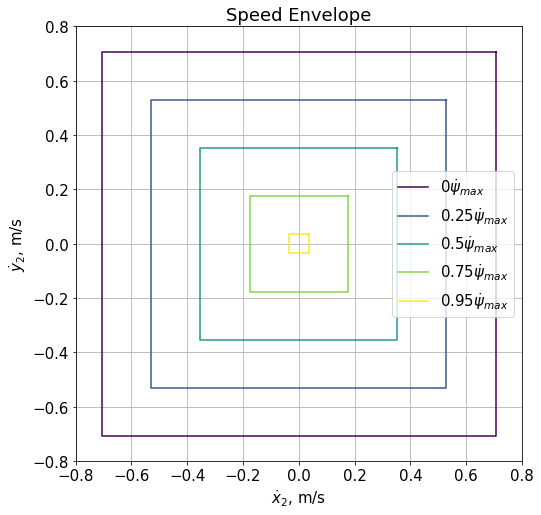
\includegraphics[width=.5\linewidth]{speed_envelope}
	\captionof{figure}{Speed Envelope}
	\label{fig:speed_envelope}
\end{figure}

\section*{Proyection of the equation}

As we know from the work of Iñigo, we can describe the Omnibot system dynamics as
\begin{gather}
	\vec H \ddot \q_r+ \vec K \dot \q_r=\R_{\psi}\R ^T\Torque \label{eq:solution}
\end{gather}
Where:
\begin{gather}
	\vec H = \mat{ m+\frac{4\,I_w}{r^2} & 0 & 0 \\ 0 & m+\frac{4\,I_w}{r^2} & 0 \\ 0 & 0 & I_z+\frac{4\,I_w\,{\left(L+l\right)}^2}{r^2} } \label{eq:H}
	\\
	\vec K = \mat{ 0 & \frac{4\,I_w\,\dot \psi }{r^2} & 0 \\ -\frac{4\,I_w\,\dot \psi }{r^2} & 0 & 0 \\ 0 & 0 & 0 }
\end{gather}

By definition: $ \dot{\q}_2  = \R_{\psi}^T \dot{\q_r}\ ,\ \ddot{\q}_2 = \R_{\psi}^T \ddot{\q_r}$

Which means that also $ \dot{\q}_r  = \R_{\psi} \dot{\q_2}\ ,\ \ddot{\q}_r = \R_{\psi} \ddot{\q_2}$

So we can rewrite the system's equation as
$$	\vec H \R_{\psi} \ddot{\q_2}+ \vec K \R_{\psi} \dot{\q_2}=\R_{\psi}\R ^T\Torque$$

Multiplying the whole equation rightside by $\R_{\psi}^T$, we get:
$$ \R_{\psi}^T	\vec H \R_{\psi} \ddot{\q_2}+ \R_{\psi}^T \vec K \R_{\psi} \dot{\q_2}=\R ^T\Torque$$
Operating, we find that $\R_{\psi}^T	\vec H \R_{\psi} = \vec{H}$ and $\R_{\psi}^T \vec{K} \R_{\psi} = \vec{K}$, so our equation proyected on axes 2 becomes:
\begin{gather}
\vec H \ddot \q_2+ \vec K \dot \q_2=\R ^T\Torque \label{eq:axes_2_eq}
\end{gather}
We can use this equation to gain more insight on the nature of the system.

\section*{Electric power}
\subsection*{Constant movement without rotation}
Let's start by assuming a straight uniform movement without rotation:
$$ \dot{\q_2} = \left[\begin{matrix}\dot{x}_{2}\\\dot{y}_{2}\\0\end{matrix}\right]\ ,\ \dot{\q_w} = \R \dot{\q_2} = \frac{\sqrt{2}}{r} \left[\begin{matrix}\dot{x}_{2}\\\dot{y}_{2}\\\dot{y}_{2}\\\dot{x}_{2}\end{matrix}\right]$$

We remember that the electric motor model looks like this:
$$ V = K_m N\dot{\phi} + Ri$$
$$ \tau_m = N K_ei\mu_{trans} - \tau_r$$
$$ \tau_r = a \dot{\phi} + b·sign(\dot{\phi}) $$
And that in straight constant movement the torque output is zero, so that the electric power consumed in a motor is 
$$ P_m = 0.301 \operatorname{sign}^{2}\left(\dot{\phi}\right) + 0.638 \operatorname{sign}\left(\dot{\phi}\right) \dot{\phi} + 0.016 \dot{\phi}^{2}$$
We can add the power consumed by all four motors to get 
$$P_tot = 0.6 \operatorname{sign}^{2}\left(\dot{x}_{2}\right) + 27.05 \operatorname{sign}\left(\dot{x}_{2}\right) \dot{x}_{2} + 0.6 \operatorname{sign}^{2}\left(\dot{y}_{2}\right) + 27.05 \operatorname{sign}\left(\dot{y}_{2}\right) \dot{y}_{2} + 14.17 \dot{x}_{2}^{2} + 14.17 \dot{y}_{2}^{2}$$

Which we can plot over $\dot{x_2}$ and $\dot{y_2}$: 
\begin{figure}[h]
	\centering
	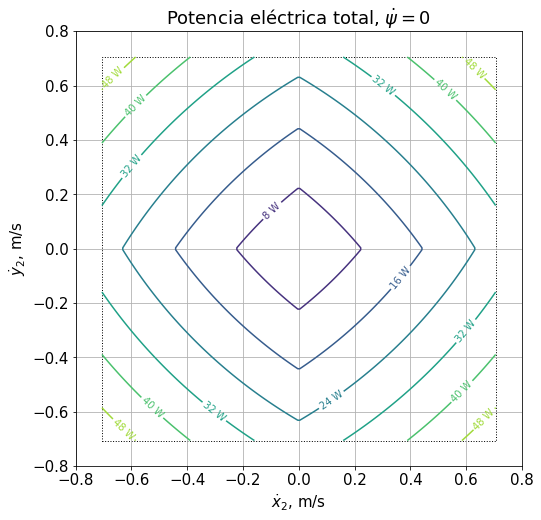
\includegraphics[width=.5\linewidth]{power_map_base_2}
	\captionof{figure}{Total electric power required to keep constat speed}
	\label{fig:power_ct_speed}
\end{figure}

We can observe that movement is most efficient in the $x_2$ and $y_2$ directions, when only two motors are running, while the least efficient directions are rotated 45 degrees respect to them: the symmetry axes of the robot.
\subsection*{Constant movement with rotation}
If our robot keeps a straight movement with constant rotation rate:
$$ \ddot{\q_2} = \vec{0}\ ,\ \dot{\q_2} = \left[\begin{matrix}\dot{x}_{2}\\\dot{y}_{2}\\\dot{\psi}\end{matrix}\right]\ ,\ \dot{\q_w} = \R \dot{\q_2} = \frac{\sqrt{2}}{r} \left[\begin{matrix}- L_{2} \dot{\psi} + \dot{x}_{2}\\L_{2} \dot{\psi} + \dot{y}_{2}\\- L_{2} \dot{\psi} + \dot{y}_{2}\\L_{2} \dot{\psi} + \dot{x}_{2}\end{matrix}\right]$$

Subtituting in the General equation:

$$\vec H \ddot \q_2+ \vec K \dot \q_2=\vec K \dot \q_2=\R ^T\Torque$$

Multiplying the equation leftside by $\R^{-1T}$:
$$\Torque=\R^{-1T}\vec K \dot \q_2 = \frac{\sqrt{2}I_w}{r}\left[\begin{matrix}\dot{\psi} \dot{y}_{2}\\- \dot{\psi} \dot{x}_{2}\\- \dot{\psi} \dot{x}_{2}\\\dot{\psi} \dot{y}_{2}\end{matrix}\right]$$

\section*{Conclusions}

We can reach maximum speed in directions parallel to the $X_{body}$ and $Y_{body}$ axes.

If we consider only the mechanical model without friction or the motors, all the energy output of the shafts are converted into kinetic energy, with independence of the advence direction.

If we consider also the motors, directions parallel to the body axes require more power than those at 45 degrees.
% Your references go at the end of the main text, and before the
% figures.  For this document we've used BibTeX, the .bib file
% scibib.bib, and the .bst file Science.bst.  The package scicite.sty
% was included to format the reference numbers according to *Science*
% style.


%\bibliography{scibib}

%\bibliographystyle{Science}



% Following is a new environment, {scilastnote}, that's defined in the
% preamble and that allows authors to add a reference at the end of the
% list that's not signaled in the text; such references are used in
% *Science* for acknowledgments of funding, help, etc.

%\begin{scilastnote}
%\item We've included in the template file \texttt{scifile.tex} a new
%environment, \texttt{\{scilastnote\}}, that generates a numbered final
%citation without a corresponding signal in the text.  This environment
%can be used to generate a final numbered reference containing
%acknowledgments, sources of funding, and the like, per {\it Science\/}
%style.
%\end{scilastnote}




% For your review copy (i.e., the file you initially send in for
% evaluation), you can use the {figure} environment and the
% \includegraphics command to stream your figures into the text, placing
% all figures at the end.  For the final, revised manuscript for
% acceptance and production, however, PostScript or other graphics
% should not be streamed into your compliled file.  Instead, set
% captions as simple paragraphs (with a \noindent tag), setting them
% off from the rest of the text with a \clearpage as shown  below, and
% submit figures as separate files according to the Art Department's
% instructions.


%\clearpage

%\noindent {\bf Fig. 1.} Please do not use figure environments to set
%up your figures in the final (post-peer-review) draft, do not include graphics in your
%source code, and do not cite figures in the text using \LaTeX\
%\verb+\ref+ commands.  Instead, simply refer to the figure numbers in
%the text per {\it Science\/} style, and include the list of captions at
%the end of the document, coded as ordinary paragraphs as shown in the
%\texttt{scifile.tex} template file.  Your actual figure files should
%be submitted separately.



\end{document}




















